\documentclass[tikz, margin=3.14mm]{standalone}
\usetikzlibrary{backgrounds}

\begin{document}
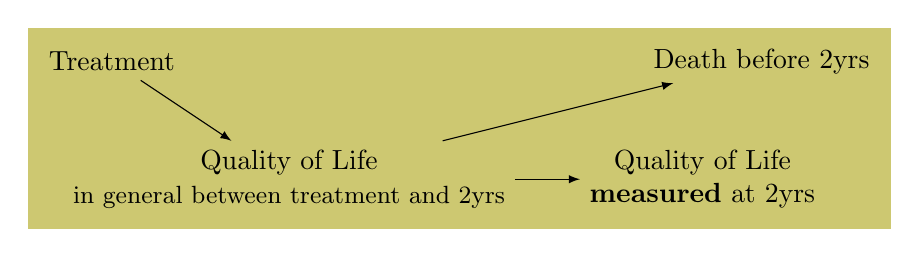
\begin{tikzpicture}[scale=3, background rectangle/.style={fill=olive!45}, show background rectangle]
    \node (z) at (0,0) {Treatment};
    \node (q1) [align=center] at (.75,-.5) {Quality of Life\\{\small in general between treatment and 2yrs}};
    \node (q2) [align=center] at (2.5,-.5) {Quality of Life\\\textbf{measured} at 2yrs};
    \node (d) at (2.75,0) {Death before 2yrs};
    
    \draw[-latex] (z) -- (q1);
    \draw[-latex] (q1) -- (q2);
    \draw[-latex] (q1) -- (d);
    \end{tikzpicture}

\end{document}